\chapter{Evaluation \& Results}
\label{ch:Evaluation and Results}

This chapter describes the evaluation tests performed on the proposed approach on the basis of developed framework. Following sections are intended to give information about input data preparation, present and discuss obtained results. To start with, the trajectories approximation using polynomial regression is considered. After that the accuracy of clustering step is tested using an aforementioned DI index. As a conclusion, output results of a classification step are discussed, validation of the anomalies detection quality is done.

\section{Evaluation of Correctness and Accuracy}

This section gives details about evaluation tests performed to validate the accuracy of obtained results.

\subsection{Trajectories Approximation Results}

To make a decision about a degree of an approximation polynomials, several experiments were run trying to fit the input trajectories into polynomials of 3\up{rd}, 4\up{th}, 5\up{th} degrees respectively. The following table depicts minimum and average values of $R^2$ metric for each of the experiments (Table \ref{table:r2_res}). 

\begin{table}[h!]
	\caption{$R^2$ values for different degrees of polynomials}
	\label{table:r2_res}
	
	\setlength{\tabcolsep}{10pt}
	\centering
	\begin{tabular}[c]{|| C{2cm} | C{2cm} C{2cm} | C{2cm} C{2cm} ||} 
		\hline
		\multirow{3}{7em}{Degrees of polynomials} 	& \multicolumn{4}{c||}{$R^2$ score} \\[1ex]\cline{2-5}
		& \multicolumn{2}{c|}{X}	& \multicolumn{2}{c||}{Y} \\ [0.5ex]
		& min 	& avg				& min 	& avg \\ [0.5ex]
		\hline \hline
		\rowcolor{nogray} \multicolumn{5}{||c||}{$1.txt$ (before filtering)} \\ [0.5ex]
		\hline
		\{3\} 							& 0.66 	& 0.994 & 0.466 & 0.989 \\ [2ex]
		\rowcolor{backgray} \{3, 4\} 	& 0.897 & 0.998 & 0.823 & 0.994 \\ [2ex]
		\{3, 4, 5\} 					& 0.949 & 0.998 & 0.864 & 0.995 \\ [2ex]
		
		\hline \hline
		\rowcolor{nogray} \multicolumn{5}{||c||}{$1.txt$} \\ [0.5ex]
		\hline
		\{3\} 							& 0.689 & 0.997 & 0.777 & 0.995 \\ [2ex]
		\rowcolor{backgray} \{3, 4\} 	& 0.942 & 0.999 & 0.872 & 0.997 \\ [2ex]
		\{3, 4, 5\} 					& 0.98 	& 0.999 & 0.88 	& 0.997 \\ [2ex]
		
		\hline \hline
		\rowcolor{nogray} \multicolumn{5}{||c||}{$2.txt$} \\ [0.5ex]
		\hline
		\{3, 4\} 						& 0.992 & 0.9997 & 0.832 & 0.996 \\ [2ex]
		\hline \hline
		
		\rowcolor{nogray} \multicolumn{5}{||c||}{$3.txt$} \\ [0.5ex]
		\hline
		\{3, 4\} 						& 0.815 & 0.995 & 0.867 & 0.996 \\ [2ex]
		\hline \hline
		
		\rowcolor{nogray} \multicolumn{5}{||c||}{$4.txt$} \\ [0.5ex]
		\hline
		\{3, 4\} 						& 0.879 & 0.995 & 0.722 & 0.993 \\ [2ex]
		\hline
	\end{tabular}
\end{table}
\todo{Last column formatting...}

This paragraph will discuss results of experiments using trajectories from first intersecton ($1.txt$) before and after filtering the trajectories. It can be seen from the Table \ref{table:r2_res} that the average values of $R^2$ score are acceptable for all the experiments. However, the minimum $R^2$ values, which are equal to 0,66 and 0,466 for the first experiment with only 3\up{rd}-degree polynomials for unfiltered trajectories, are poor and unsatisfactory, meaning that model can predict barely half of the points for some trajectories correctly. Filtering out trajectories with short displacements in terms of both space and time improved the results significantly. However, results for approximation using 3\up{rd}-degree polynomials are still insufficient. This can affect following analysis and worsen further analysis. For that reason approximation using several degrees was performed in a following way: 
\begin{enumerate}
	\item firstly perform approximation using the lowest degree of a polynomial as a starting point,
	\item compare the obtained $R^2$ with a predefined threshold (0,98 in this case); if the obtained value is less than the threshold value, increase the degree and reperform polynomial regression,
	\item continue till the acceptable $R^2$ is obtained or till reaching the limit for a polynomial degree to check (5 in this case). 
\end{enumerate} 

Approximation using 3\up{rd} and 4\up{th} degree polynomials in conjunction improved both minimum and average values of $R^2$ drastically. Though adding a 5\up{th} degree polynomial into consideration did not affect results significantly and improved the average coefficient only for 0,01 in comparison with the previous experiment. In view of this it was decided to focus on approximation using 3\up{rd} and 4\up{th} degrees and run the experiments on the rest of input trajectories data sets ($2.txt$, $3.txt$, $4.txt$).

For the sake of simplicity the trajectories are classified into two groups depending on a degree of polynomials used to approximate: first group contains trajectories approximated with a 3\up{rd} degree polynomial functions while the second group consists of trajectories approximated with a 4\up{th} degree polynomial functions. Both groups were analyzed in terms of a shape and an average speed. Figure \ref{fig:regr-pol-4} depicts second group of trajectories and Table \ref{table:speeds} gives the minimum, average and maximum speed of trajectories for both groups.

\begin{figure}
	\centering
	\begin{subfigure}[b]{0.3\textwidth}
		\centering{}
		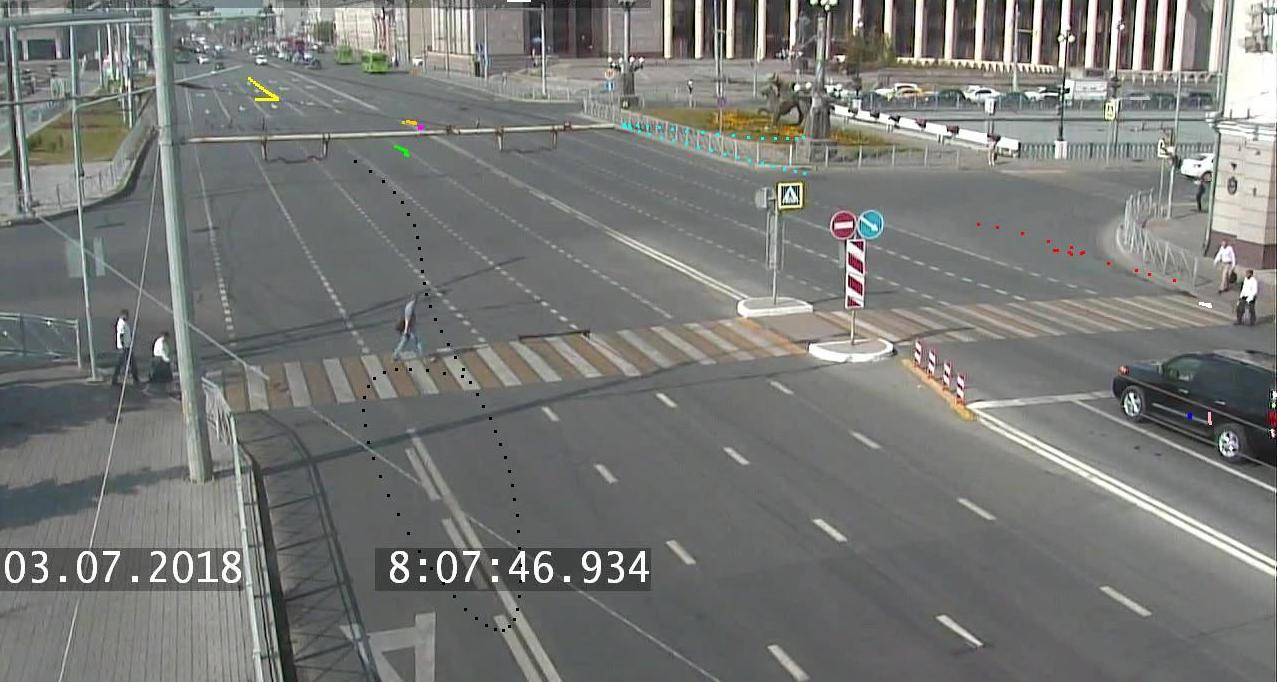
\includegraphics[width=\textwidth]{images/regr_1_pol_4.jpg}
		\caption{$1.txt$}
		\label{fig:regr-1-pol-4}
	\end{subfigure}
	\hfill
	\begin{subfigure}[b]{0.3\textwidth}
		\centering{}
		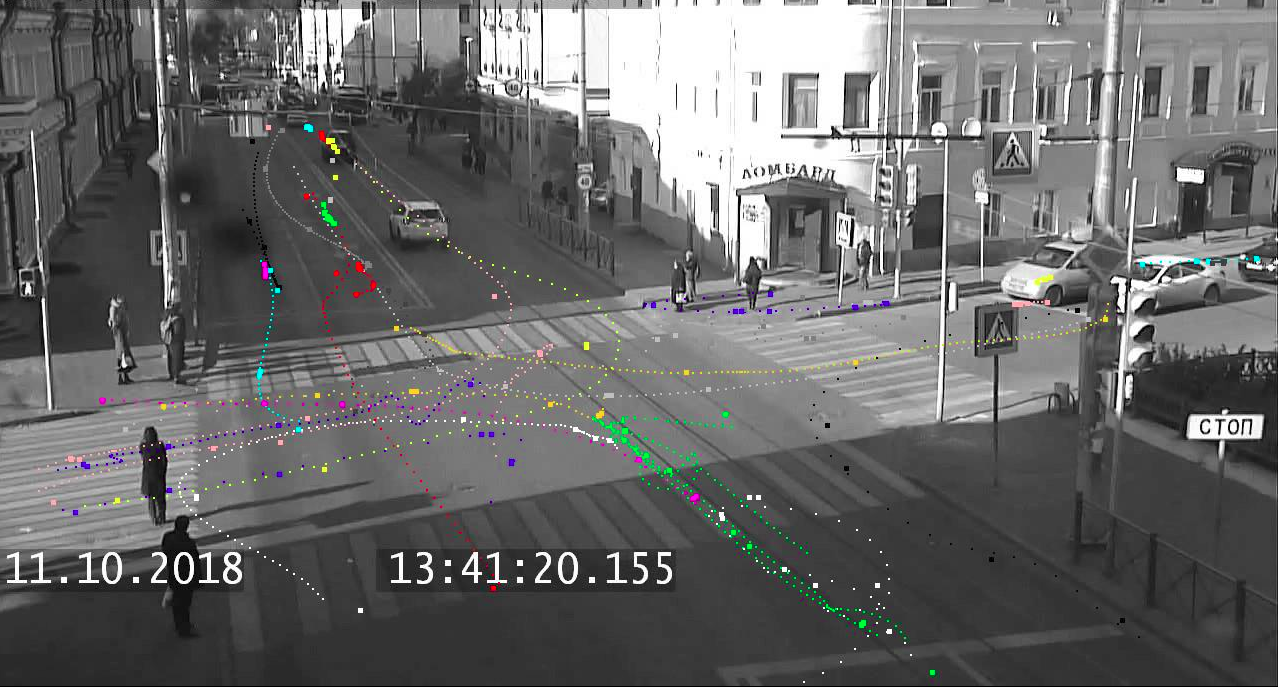
\includegraphics[width=\textwidth]{images/regr_3_pol_4.png}
		\caption{$3.txt$}
		\label{fig:regr-3-pol-4}
	\end{subfigure}
	\hfill
	\begin{subfigure}[b]{0.3\textwidth}
		\centering{}
		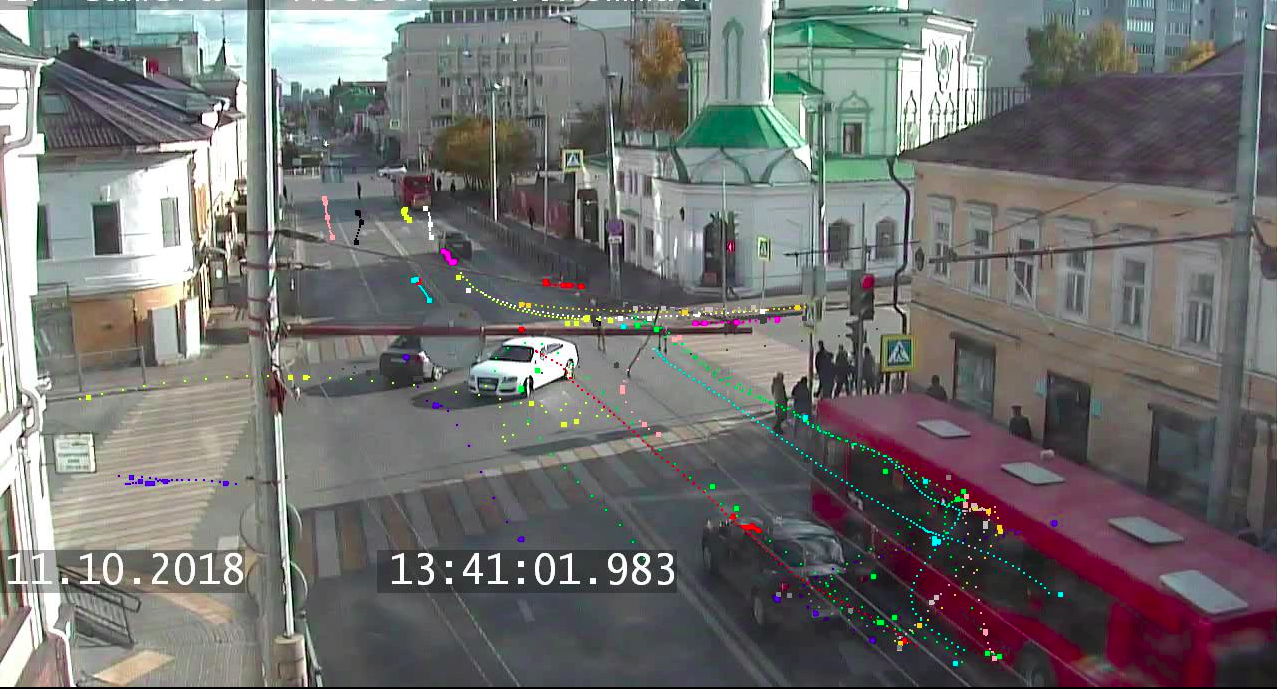
\includegraphics[width=\textwidth]{images/regr_4_pol_4.png}
		\caption{$4.txt$}
		\label{fig:regr-4-pol-4}
	\end{subfigure}
	\caption{Trajectories approximated with 4\up{th}-degree polynomial functions}
	\label{fig:regr-pol-4}
\end{figure}

\begin{table}[h!]
	\caption{Overview of min, avg and max speeds of vehicles}
	\label{table:speeds}
	
	\setlength{\tabcolsep}{10pt}
	\centering
	\begin{tabular}[c]{|| C{2.5cm} | C{2.5cm} C{2.5cm} C{2.5cm} ||} 
		\hline
		\multirow{2}{7em}{Degree of a polynomial} 	
		& \multicolumn{3}{c||}{Speed \textit{(pixels per sec)}} \\[1ex]\cline{2-4}
		& min 		& avg		& max 				\\ [2ex]
		
		\hline \hline
		\rowcolor{nogray} \multicolumn{4}{||c||}{$1.txt$ (before filtering)} 	\\ [0.5ex]
		\hline
		\rowcolor{backgray} \{3\} 	& 18.555 	& 335.365 	& 1721.499 			\\ [2ex]
		
		\rowcolor{backgray} \{4\} 	& 1.206		& 72.34 	& 374.396 			\\ [2ex]
		\hline
		
		\rowcolor{nogray} \multicolumn{4}{||c||}{$1.txt$} 	\\ [0.5ex]
		\hline
		\rowcolor{backgray} \{3\} 	& 61.814 	& 372.435 	& 909.121 			\\ [2ex]
		
		\rowcolor{backgray} \{4\} 	& 26.603	& 229.053 	& 602.773 			\\ [2ex]
		
		\hline
		\rowcolor{nogray} \multicolumn{4}{||c||}{$2.txt$} 	\\ [0.5ex]
		\hline
		\{3\} 	& 85.705 	& 494.016 	& 1107.96 			\\ [2ex]
		
		\{4\} 	& 183.087	& 613.865 	& 900.737 			\\ [2ex]
		\hline
		
		\rowcolor{nogray} \multicolumn{4}{||c||}{$3.txt$} 	\\ [0.5ex]
		\hline
		\{3\} 	& 13.65 	& 301.481 	& 1012.748 			\\ [2ex]
		
		\{4\} 	& 29.26		& 206.119 	& 764.25 			\\ [2ex]
		\hline
		
		\rowcolor{nogray} \multicolumn{4}{||c||}{$4.txt$} 	\\ [0.5ex]
		\hline
		\{3\} 	& 43.01 	& 269.074 	& 872.33	 		\\ [2ex]
		
		\{4\} 	& 22.92		& 163.431 	& 708.154 			\\ [2ex]
		\hline
		
	\end{tabular}
\end{table}

Thereinafter the trajectories approximated with 3\up{rd}- and 4\up{th}-degree polynomial functions will be referred to as a first and second groups of trajectories respectively. It can be observed that trajectories approximated with 3\up{rd}- and 4\up{th}-degree polynomial functions have the widely different speeds. The first group includes trajectories with much higher speeds, particularly striking is that the maximum speed for the second group is almost equal to average speed for the first group and the average speed for the first group is almost four times as much as for the second group for the case of unfiltered trajectories. After excluding the short trajectories from the consideration results became more smooth, however the same observation still takes place and is still noticeable. Also the picture depicts that 4\up{th}-degree polynomial functions were used to approximate trajectories of complex shape or trajectories with densely located trajectory points. 

Such a tendency is mostly distinguishable while considering trajectories from the first intersection, which can supposed to be the representative set of trajectories since it has the largest amount of data instances. It is also worth noting that the second trajectories data set ($2.txt$) has only 10 trajectories in the first group, hence the trajectories speed analysis can not be very accurate.

\subsubsection{Summary}

Hence, it follows up that the higher-order polynomial functions are preferred to approximate trajectories of following groups:
\begin{itemize}
	\item slow-moving or inactive vehicle trajectories (including trajectories of vehicles waiting at the intersections), detectable on Figure \ref{fig:regr-1-pol-4};
	\item vehicle trajectories with a non-constant speed or an acceleration on some sections of a path (can be represented by non-equal allocation of trajectory points, where dense areas of trajectory points signalize about acceleration during these time intervals; as a result low-order polynomial can not describe such a complex dependency between a coordinate and a time);
	\item trajectories of complex shapes (sharp turns, Pascal snails), especially recognizable on Figures \ref{fig:regr-pol-4}b-c.
\end{itemize}
